\chapter{Planning}

\section{Risk Analysis}

The main purpose of this system will be providing a tool for people to test computational model, researchers can use this system to test if the model is working as intended and company or others who want to use the model can use it to see the model’s accuracy. The following are the stake holder of this project:\\*

1.	Developers of the Causcumber project

2.	Researchers who will be using Causcumber to test their model

3.	Organization that uses this tool to check their model’s accuracy
\\*
\\*
One of the main goals of this model is to return a clear and correct result for the user, if the returned result is incorrect or misleading. This might affect the development of the computational models that use this tool for testing, the result might end up being inaccurate and people who uses these results for scientific research or other purpose may affect by this mistake. 

\section{Project Plan}

For this project, I plan to start with understand the how Causcumber work, what kind of result does it produce. Then, following by understand how behave and cucumber function in the system, by understand how these tool works, it would benefit a lot for future plan. \\*
The next phase will be designing the user interface for Causcumber, this phase will be focus on design the user interface and making sure it is easy to understand, and easy to operate. \\*
After the design the is done, I plan start implement the system, combine the system with the interface, in this phase will be working in Scrum method, where the project will focus on rapidly adding or change function based on feedback, this is the current phase where the project is in right now, a list of features is either being implanting or will be implement in the near future. \\*
The last phase will be polishing the system, focusing on debugging, and making sure the system runs smooth. 

\section{Current progress}

This project already has some progress, I already have grasp on how Causcumber work and have move into the scrum phase where a user interface being develop and adding or adjust functions according to feedback, below will be some figure showing the current progress of the system:
\begin{center}
	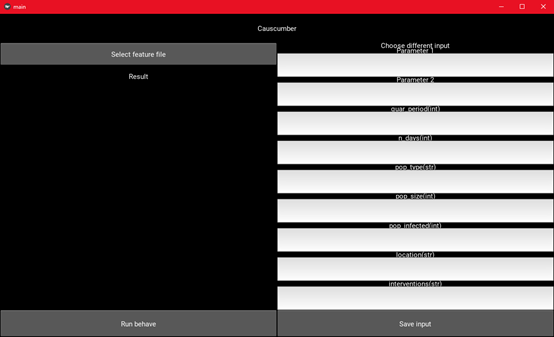
\includegraphics[width=8cm]{figures/Gui_overview.png}\\
	Figure 3. An overview of the user interface
\end{center}
This is an overview of the user interface, the left part will display the result, and the right part is where the users can custom their feature file.
\begin{center}
	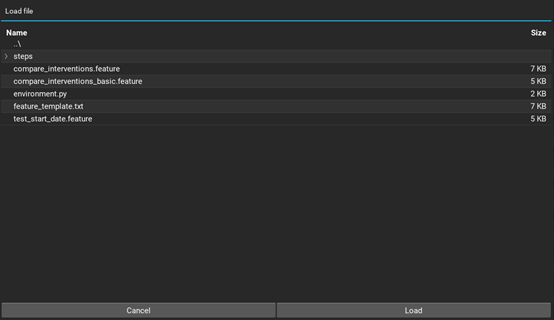
\includegraphics[width=8cm]{figures/select_feature_file.png}\\
	Figure 4. Select feature file screen
\end{center}
User can select which feature file they want to execute, then Causcumber will load and produce the result into a xml file.
\begin{center}
	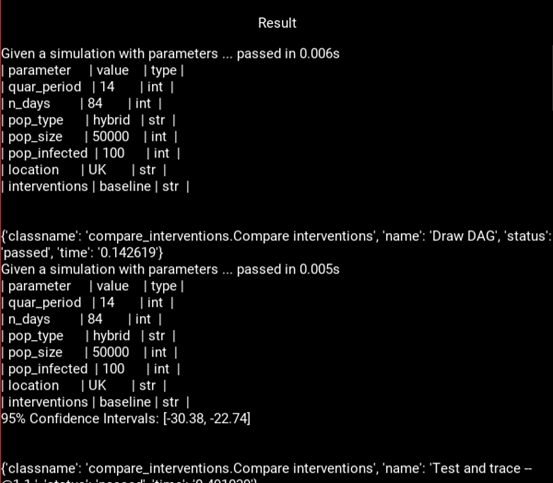
\includegraphics[width=8cm]{figures/Result_display.png}\\
	Figure 5. Result produced by Causcumber and display in the result section
\end{center}
After Causcumber load the feature file and produce to the xml file, the user interface can read from the xml file, retrieve the useful information and remove the unwanted ones, users can view the input parameters and how accurate a parameter in the computational models are.
\begin{center}
	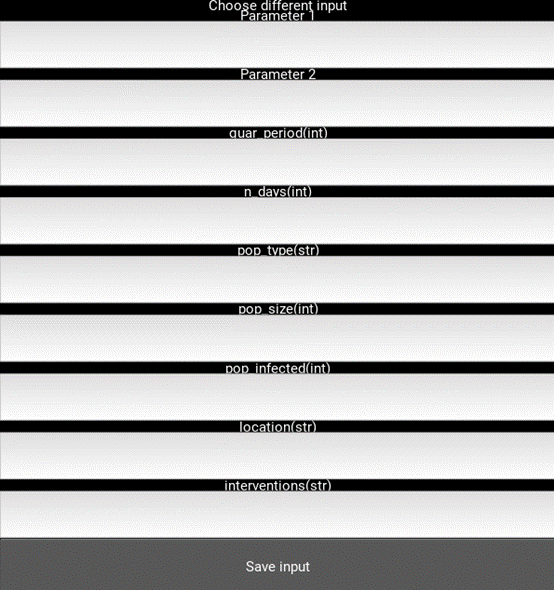
\includegraphics[width=8cm]{figures/Input_section.png}\\
	Figure 6. Choose different input value, and save it into a feature file
\end{center}
In the right side of the interface, user can create their own feature file with their own parameter to test the system, the system will compile the input value and save as a new feature file.
